%% ======================================================================
%%  IEEE journal paper (IEEEtran, journal mode)
%%
%%  Build:  pdflatex IEEE_paper -> bibtex IEEE_paper -> pdflatex x2
%%  Overleaf: upload this folder (IEEE_paper.tex, references.bib, figures/),
%%            compiler = pdfLaTeX.
%%
%%  Every number in this paper is produced by the scripts in scripts/
%%  (run_inference.py, run_baselines.py, find_duplicates.py,
%%  analyze_leakage.py, make_figures.py) from the trained model
%%  models/taka_authenticator.pth and the public JaalTaka dataset.
%% ======================================================================

\documentclass[journal]{IEEEtran}

\usepackage{cite}
\usepackage{amsmath,amssymb,amsfonts}
\usepackage{graphicx}
\usepackage{booktabs}
\usepackage{adjustbox}
\usepackage{multirow}
\usepackage{array}
\usepackage{tabularx}
\usepackage{algorithm}
\usepackage{algpseudocode}
\usepackage{url}
\usepackage{xcolor}
\usepackage[hidelinks,
  pdftitle={Reliable Smartphone-Based Detection of Counterfeit Bangladeshi Banknotes},
  pdfauthor={Debobrato Biswas, Imran Mahmud}]{hyperref}

\graphicspath{{figures/}}
\newcolumntype{L}[1]{>{\raggedright\arraybackslash}p{#1}}
\newcolumntype{C}[1]{>{\centering\arraybackslash}p{#1}}
\hyphenation{bank-note bank-notes counter-feit counter-feits Efficient-Net}

\begin{document}

\title{Reliable Smartphone-Based Detection of Counterfeit Bangladeshi Banknotes:
Multi-View Deep Learning with Out-of-Distribution Rejection and a Benchmark Audit}

\author{Debobrato~Biswas and Imran~Mahmud%
\thanks{D. Biswas and I. Mahmud are with the Department of Software Engineering,
Daffodil International University, Dhaka 1207, Bangladesh.}%
\thanks{Corresponding author: Debobrato Biswas (e-mail: biswas2305343003@diu.edu.bd).}}

\markboth{Reliable Smartphone-Based Detection of Counterfeit Bangladeshi Banknotes}%
{Biswas and Mahmud: Reliable Smartphone-Based Detection of Counterfeit Bangladeshi Banknotes}

\maketitle

%% ----------------------------------------------------------------------
\begin{abstract}
Counterfeit high-value banknotes harm retailers and individuals who cannot afford
dedicated verification hardware. This paper presents a smartphone-based authentication
system for Bangladeshi Tk~500 and Tk~1000 notes and evaluates it on JaalTaka, a public
benchmark of 1{,}390 notes (802 genuine and 588 counterfeit notes seized by law
enforcement) with six photographs per note. The system fine-tunes an ImageNet-pretrained
EfficientNet-B0, fuses the predictions of up to six photographs of the same note, and
returns a three-way verdict (genuine, uncertain, or counterfeit) with an adjustable
strictness threshold. A Mahalanobis-plus-residual test in the network's embedding space
rejects photographs that do not resemble the supported notes, and Grad-CAM heatmaps show
which regions drove each decision. On a held-out test set of 208 notes that share no note
with training, the system reaches 98.08\% note-level accuracy (95\% CI 95.16--99.25\%)
and an ROC-AUC of 0.994. It runs at 37~ms per photograph on a desktop CPU. An audit of the
benchmark shows why these figures must be read with care. Pixel-level matching groups the
1{,}390 notes into only 846 distinct photograph sets: 116 of the 208 test notes have an
exact or augmented copy in the training or validation split, and 12 duplicate groups carry
\emph{both} labels. All four test errors fall in these label-conflict groups. On the 92 test
notes without any copy in training, the system makes no errors, but so do a
1-nearest-neighbour classifier and a linear probe on frozen ImageNet features. The
benchmark is therefore saturated under note-level splitting. We release the duplicate
groups and recommend group-aware splits and counterfeit-family hold-out tests for future
work.
\end{abstract}

\begin{IEEEkeywords}
Banknote authentication, Bangladeshi Taka, counterfeit detection, data leakage,
EfficientNet, explainable AI, Grad-CAM, out-of-distribution detection, transfer learning.
\end{IEEEkeywords}

%% ======================================================================
\section{Introduction}
\label{sec:intro}

\IEEEPARstart{C}{ounterfeit} banknotes undermine trust in cash, which remains the main
means of payment for small retailers and much of the population in Bangladesh. The
Tk~500 and Tk~1000 notes are the preferred targets of counterfeiters because a single
accepted forgery causes a large loss. Banks use sorting machines with ultraviolet,
infrared, and magnetic sensors. Shopkeepers, transport workers, and ordinary citizens,
however, rely on visual and tactile checks of the watermark, security thread, and
intaglio print, which are slow and unreliable for untrained users. A smartphone camera is
the one sensor almost everyone carries, which makes image-based authentication on
commodity devices an attractive complement to manual checks.

Earlier image-based counterfeit detectors relied on hand-crafted features such as
luminance histograms~\cite{yeh2011}, background printing texture~\cite{berenguel2016}, or
specific security features~\cite{uddin2016}, often under controlled scanner or
multispectral imaging~\cite{baek2018}. Convolutional neural networks (CNNs) trained on
smartphone photographs have since been shown to detect forgeries of several
currencies~\cite{pham2020,pham2022}. For Bangladeshi currency, most published work
addressed denomination recognition~\cite{jahangir2007,linkon2020}. The recent JaalTaka
dataset~\cite{piyas2025jaaltaka} made counterfeit detection research possible by
releasing smartphone photographs of genuine notes and of counterfeits seized by the
Rapid Action Battalion (RAB). Its authors reported test accuracies of 97.4--98.9\% for
five ImageNet CNNs.

High accuracy on a benchmark is necessary, but not sufficient, for a tool that people
will trust with money. A deployable system must also (i)~behave sensibly when the input
is not a supported note, (ii)~admit uncertainty instead of forcing a binary answer,
(iii)~explain its decision, and (iv)~be evaluated in a way that predicts its behaviour on
notes it has never seen. The last point is easy to get wrong. Deep networks readily
exploit shortcuts~\cite{geirhos2020shortcut}, and duplicated or near-duplicated samples
across training and test splits silently inflate reported accuracy, a problem that has
affected many applied machine-learning studies~\cite{kapoor2023leakage}.

This paper addresses these requirements. Its contributions are as follows.
\begin{enumerate}
\item A complete, open, CPU-real-time authentication pipeline for Tk~500 and Tk~1000
notes (Fig.~\ref{fig:pipeline}). It combines an EfficientNet-B0~\cite{tan2019efficientnet}
classifier, fusion of up to six photographs of one note, a three-way decision rule with
an adjustable strictness threshold, an embedding-space out-of-distribution (OOD) gate,
and Grad-CAM~\cite{selvaraju2017gradcam} explanations.
\item A note-disjoint evaluation on JaalTaka that reports confidence intervals,
per-photograph and per-note results, threshold behaviour, OOD rejection rates, and
comparisons with frozen-feature baselines.
\item An audit of the benchmark using pixel-level duplicate matching. It reveals that
most test notes have copies in the training split and that several duplicate groups
carry contradictory labels. It also shows that every test error of our system is caused
by such a label conflict, and that the benchmark is saturated once duplicates are
controlled. An occlusion test further indicates that part of the discriminative signal
lies outside the note's central region.
\end{enumerate}

The remainder of the paper is organised as follows. Section~\ref{sec:related} reviews
related work. Section~\ref{sec:data} describes the dataset and protocol, and
Section~\ref{sec:method} the proposed system. Section~\ref{sec:results} reports the
experiments and the benchmark audit. Section~\ref{sec:discussion} discusses limitations,
and Section~\ref{sec:conclusion} concludes the paper.

%% ======================================================================
\section{Related Work}
\label{sec:related}

\subsection{Hand-Crafted Counterfeit Detection}
Early systems extracted engineered features from images captured under controlled
conditions. Yeh~\textit{et~al.}~\cite{yeh2011} classified luminance histograms of
Taiwanese banknotes with multiple-kernel support vector machines (SVMs).
Berenguel~\textit{et~al.}~\cite{berenguel2016} analysed the fine background printing
texture captured by a flatbed scanner, which differs between the intaglio and offset
printing of genuine notes and the inkjet or laser printing of most forgeries.
Baek~\textit{et~al.}~\cite{baek2018} exploited multispectral images, in which genuine
inks respond differently from counterfeit ones. For Bangladeshi currency,
Uddin~\textit{et~al.}~\cite{uddin2016} inspected individual security features in
banknote images. Dittimi and Suen~\cite{dittimi2018} brought counterfeit detection to a
mobile application. These methods are interpretable and light, but they depend on
controlled imaging and on carefully tuned features for each currency and denomination.

\subsection{Deep Learning for Banknotes}
Transfer learning from ImageNet~\cite{deng2009imagenet,yosinski2014transferable}
allows CNNs to be trained with the few thousand images that are typically available for
banknotes. Pham~\textit{et~al.} detected fake banknotes from visible-light smartphone
images to assist visually impaired users~\cite{pham2020} and later studied the
cross-dataset setting for multinational banknotes~\cite{pham2022}. For Bangladeshi notes,
Jahangir and Chowdhury~\cite{jahangir2007} used a neural network for denomination
recognition, and Linkon~\textit{et~al.}~\cite{linkon2020} combined lightweight CNNs with
transfer learning for denomination detection. Counterfeit detection on the JaalTaka
dataset was first benchmarked by its authors~\cite{piyas2025jaaltaka} with
DenseNet121~\cite{huang2017densenet}, ResNet50~\cite{he2016resnet},
VGG16~\cite{simonyan2015vgg}, MobileNetV2~\cite{sandler2018mobilenetv2}, and
InceptionV3~\cite{szegedy2016inception}, and transfer learning has also been applied
to counterfeit Bangladeshi notes in~\cite{tabassum2025}. Table~\ref{tab:related}
summarises these studies. None of them evaluates OOD inputs, uncertainty, or the
duplicate structure of the data.

\begin{table*}[!t]
\caption{Representative Banknote Authentication Studies}
\label{tab:related}
\centering
\footnotesize
\begin{tabularx}{\textwidth}{@{}L{2.9cm}L{1.9cm}L{3.1cm}X@{}}
\toprule
Study & Currency & Imaging & Approach and task \\
\midrule
Yeh \textit{et~al.}~\cite{yeh2011} (2011) & Taiwan dollar & Image sensor & Luminance histograms + multiple-kernel SVM; counterfeit detection \\
Berenguel \textit{et~al.}~\cite{berenguel2016} (2016) & Banknotes & Flatbed scanner & Background printing-texture features + SVM; counterfeit detection \\
Uddin \textit{et~al.}~\cite{uddin2016} (2016) & BDT & Camera images & Image-based analysis of security features; counterfeit detection \\
Baek \textit{et~al.}~\cite{baek2018} (2018) & Banknotes & Multispectral & Spectral response of inks; counterfeit detection \\
Dittimi and Suen~\cite{dittimi2018} (2018) & Banknotes & Smartphone & Mobile application; counterfeit detection \\
Pham \textit{et~al.}~\cite{pham2020} (2020) & Banknotes & Smartphone, visible light & CNN; fake-banknote detection for visually impaired users \\
Linkon \textit{et~al.}~\cite{linkon2020} (2020) & BDT & Camera images & Lightweight CNN + transfer learning; denomination recognition \\
Pham \textit{et~al.}~\cite{pham2022} (2022) & USD, EUR, KRW, JOD & Smartphone & CNN; fake detection across datasets \\
Piyas \textit{et~al.}~\cite{piyas2025jaaltaka} (2025) & BDT 500/1000 & Smartphone (4 models) & JaalTaka dataset; five ImageNet CNN baselines (best 98.9\%) \\
Tabassum \textit{et~al.}~\cite{tabassum2025} (2025) & BDT & Images & Transfer learning; counterfeit detection \\
\midrule
This work & BDT 500/1000 & Smartphone, 1--6 views & EfficientNet-B0, multi-view fusion, three-way decision, OOD gate, Grad-CAM, duplicate audit \\
\bottomrule
\end{tabularx}
\end{table*}

\subsection{Reliability: OOD Detection, Explanation, and Leakage}
A classifier trained on two classes assigns one of them to any input, including
photographs of other denominations or unrelated objects. Hendrycks and
Gimpel~\cite{hendrycks2017baseline} showed that the maximum softmax probability is a
useful but weak OOD signal. Lee~\textit{et~al.}~\cite{lee2018mahalanobis} obtained
stronger detection by fitting Gaussian models to intermediate features and scoring
inputs by their Mahalanobis distance, an approach we adapt to a low-dimensional subspace.
Neural network probabilities are also often miscalibrated~\cite{guo2017calibration},
which motivates an explicit ``uncertain'' outcome instead of a single fixed threshold.
Grad-CAM~\cite{selvaraju2017gradcam} highlights the image regions that support a class
and is widely used to check what a CNN has learned. Finally,
Geirhos~\textit{et~al.}~\cite{geirhos2020shortcut} described how networks solve benchmarks
through unintended shortcuts, and Kapoor and Narayanan~\cite{kapoor2023leakage} documented
how leakage between training and test data, including duplicated samples, inflates
published results. Our audit in Section~\ref{sec:audit} applies these lessons to
counterfeit banknote detection.

%% ======================================================================
\section{Dataset and Evaluation Protocol}
\label{sec:data}

\subsection{The JaalTaka Dataset}
JaalTaka~\cite{piyas2025jaaltaka,jaaltaka_data} contains photographs of 1{,}390
Bangladeshi notes: 802 genuine notes (398 Tk~500 and 404 Tk~1000) collected from three
national banks, and 588 counterfeit notes (320 Tk~500 and 268 Tk~1000) supplied by RAB
for research. Each note was photographed six times with one of four smartphones (Samsung
Galaxy A50 and M31, Redmi Note~8 and Note~9~Pro), giving 8{,}340 images. The six photographs
cover different segments of the front and back of the note (Fig.~\ref{fig:samples}). The
dataset description states that 649 original notes (502 genuine and 147 counterfeit) were
expanded to 1{,}390 by augmentation. We resized every image so that its longer side is
1{,}024 pixels; the data are distributed under the CC~BY~4.0 licence.

\begin{figure*}[!t]
\centering
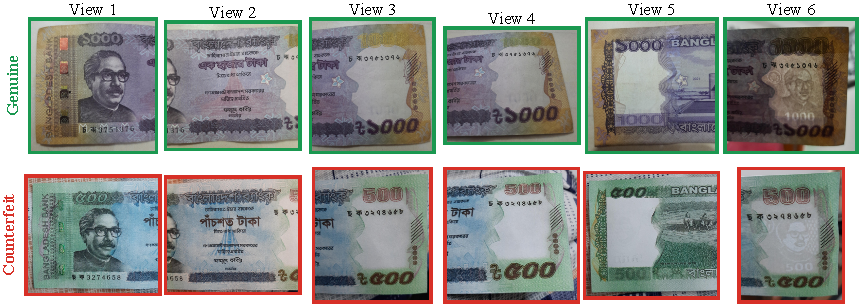
\includegraphics[width=\textwidth]{fig_samples}
\caption{The six photographs of one genuine Tk~1000 note (top) and one counterfeit
Tk~500 note (bottom) from the JaalTaka test split. Each view shows a different segment
of the note; the colour, lighting, and background vary with the phone and the session.}
\label{fig:samples}
\end{figure*}

\subsection{Note-Disjoint Split}
Because the six photographs of a note are strongly correlated, we split the data by
note, never by photograph. Within each class, notes were shuffled with a fixed seed (42)
and assigned 70\%/15\%/15\% to training, validation, and test, so that no note
contributes photographs to more than one split. Table~\ref{tab:split} lists the result.
The validation split is used for model selection and to calibrate the OOD gate; the
test split is used once, for the results in Section~\ref{sec:results}. As
Section~\ref{sec:audit} shows, a note-disjoint split is \emph{not} sufficient on this
dataset, because distinct note identifiers can share the same photographs.

\begin{table}[!t]
\caption{Note-Disjoint Split of JaalTaka (Seed 42)}
\label{tab:split}
\centering
\footnotesize
\setlength{\tabcolsep}{4pt}
\begin{adjustbox}{max width=\columnwidth}
\begin{tabular}{@{}lrrrrr@{}}
\toprule
& \multicolumn{3}{c}{Notes} & \multicolumn{2}{c}{Photographs} \\
\cmidrule(lr){2-4}\cmidrule(l){5-6}
Split & Genuine & Counterf. & Total & Genuine & Counterf. \\
\midrule
Training   & 562 & 412 & 974 & 3{,}372 & 2{,}472 \\
Validation & 120 &  88 & 208 &   720   &   528   \\
Test       & 120 &  88 & 208 &   720   &   528   \\
\midrule
Total      & 802 & 588 & 1{,}390 & 4{,}812 & 3{,}528 \\
\bottomrule
\end{tabular}
\end{adjustbox}
\end{table}

%% ======================================================================
\section{Proposed System}
\label{sec:method}

Fig.~\ref{fig:pipeline} shows the processing chain. A user photographs one note one to
six times. Each photograph is classified independently. Photographs that fail the OOD
gate are discarded, the remaining probabilities are averaged, and a three-way decision
is made. A Grad-CAM heatmap accompanies every photograph.

\begin{figure*}[!t]
\centering
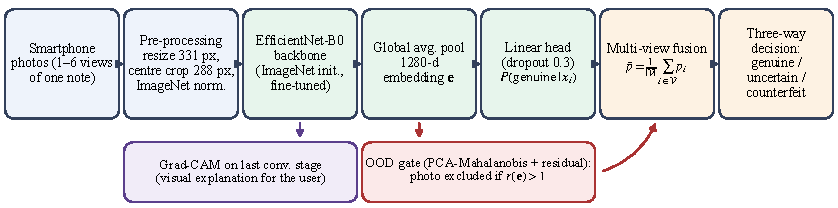
\includegraphics[width=\textwidth]{fig_pipeline}
\caption{Overview of the proposed system. Each photograph $x_i$ of a note is classified
by a fine-tuned EfficientNet-B0. Photographs whose embedding $\mathbf{e}$ fails the OOD
test are excluded, the genuine probabilities of the remaining views are averaged, and
the note is labelled genuine, uncertain, or counterfeit. Grad-CAM explains each
per-photograph decision.}
\label{fig:pipeline}
\end{figure*}

\subsection{Classifier}
\label{sec:classifier}
We use EfficientNet-B0~\cite{tan2019efficientnet}, which offers a good trade-off between
accuracy and computation on CPUs and mobile devices, initialised with ImageNet
weights~\cite{deng2009imagenet}. The convolutional feature extractor $f(\cdot)$ maps an
input $x$ to a $1280\times9\times9$ feature map for $288\times288$ inputs; global average
pooling yields the embedding $\mathbf{e}=f(x)\in\mathbb{R}^{1280}$. The ImageNet classifier
is replaced by dropout ($p=0.3$) and a linear layer with two outputs, so that
\begin{equation}
p(x) = \operatorname{softmax}\!\left(\mathbf{W}\mathbf{e}+\mathbf{b}\right)_{\text{genuine}} .
\label{eq:prob}
\end{equation}
The model has 4.01~M parameters.

\subsection{Training}
\label{sec:training}
Training images are augmented with random resized crops (scale 0.35--1.0, aspect ratio
0.75--1.33, output $288\times288$), rotations of up to $\pm10^\circ$, colour jitter
(brightness and contrast $\pm0.4$, saturation $\pm0.3$, hue $\pm0.04$), and, with
probability 0.2, Gaussian blur. The augmentations encourage the network to rely on
print and texture rather than lighting, framing, or background. At evaluation, the
shorter image side is resized to 331 pixels and the central $288\times288$ region is
kept, which removes most of the background.

The first four stages of EfficientNet-B0 (the stem and the first three MBConv stages),
which compute generic edge and colour filters, are frozen, and their batch-normalisation
statistics are kept from ImageNet. The rest of the network is fine-tuned with the
class-weighted, label-smoothed~\cite{szegedy2016inception} cross-entropy
\begin{equation}
\mathcal{L} = -\sum_{c\in\{0,1\}} w_c\, q_c \log \hat{y}_c, \quad
q_c = (1-\varepsilon)\,\mathbb{1}[c=y] + \tfrac{\varepsilon}{2},
\label{eq:loss}
\end{equation}
where $\hat{y}$ is the softmax output, $\varepsilon=0.05$, and $w_c=N/(2N_c)$ compensates
for the 562:412 class imbalance. We use AdamW~\cite{loshchilov2019adamw} and a one-cycle
learning-rate schedule~\cite{smith2019superconvergence}; Table~\ref{tab:hyper} lists the
settings. After each epoch, the model is evaluated on the validation split, and the
weights with the highest sum of validation accuracy and AUC are kept. Validation accuracy
rose from 98.80\% after the first epoch to 99.04\%, and validation AUC from 0.9919 to
0.9976 after the sixth, which was selected. Training took about 55~min on an Intel Core
i5-12400 CPU without a GPU, using PyTorch~\cite{paszke2019pytorch}.

\begin{table}[!t]
\caption{Training Configuration}
\label{tab:hyper}
\centering
\footnotesize
\setlength{\tabcolsep}{4pt}
\begin{adjustbox}{max width=\columnwidth}
\begin{tabular}{@{}ll@{}}
\toprule
Setting & Value \\
\midrule
Backbone & EfficientNet-B0, ImageNet-1k weights \\
Frozen layers & Stem + first 3 MBConv stages \\
Head & Dropout 0.3, linear $1280\rightarrow2$ \\
Input size & $288\times288$ \\
Optimiser & AdamW, weight decay $10^{-4}$ \\
Learning rate & One-cycle, peak $3\times10^{-4}$, 15\% warm-up \\
Batch size / epochs & 12 / 6 (487 steps per epoch) \\
Loss & Weighted cross-entropy, label smoothing 0.05 \\
Model selection & Max.\ validation (accuracy + AUC) \\
Random seed & 42 (split, initialisation, shuffling) \\
\bottomrule
\end{tabular}
\end{adjustbox}
\end{table}

\subsection{Multi-View Fusion and Three-Way Decision}
\label{sec:decision}
Let $\mathcal{V}$ be the set of photographs of one note that pass the OOD gate
(Section~\ref{sec:ood}). The note-level genuine probability is the mean
\begin{equation}
\bar{p} = \frac{1}{|\mathcal{V}|}\sum_{i\in\mathcal{V}} p(x_i).
\label{eq:fusion}
\end{equation}
Averaging is simple, needs no extra training, and accepts any number of views, which
suits an interactive application in which a user may submit one quick photograph or six
careful ones; it is the late-fusion analogue of view pooling in multi-view
CNNs~\cite{su2015mvcnn}. Given a strictness threshold $\tau\in[0.5,1)$, the verdict is
\begin{equation}
\text{verdict} =
\begin{cases}
\text{not supported} & \text{if } \mathcal{V}=\emptyset,\\
\text{genuine} & \text{if } \bar{p}\ge\tau,\\
\text{counterfeit} & \text{if } \bar{p}<0.5,\\
\text{uncertain} & \text{otherwise.}
\end{cases}
\label{eq:decision}
\end{equation}
The asymmetric rule reflects the asymmetric cost of errors: accepting a counterfeit
causes a direct loss, whereas an ``uncertain'' verdict only asks the user to check the
watermark, security thread, and raised print by hand or to add photographs. The default
is $\tau=0.7$; users can choose 0.6, 0.7, or 0.85, or set any value in the interface.

\subsection{Out-of-Distribution Gate}
\label{sec:ood}
Following the feature-space approach of Lee~\textit{et~al.}~\cite{lee2018mahalanobis},
we model the embeddings of the training photographs. Let $\boldsymbol{\mu}$ be their
mean and $\mathbf{U}_k\in\mathbb{R}^{1280\times k}$ the first $k=64$ principal directions,
with variances $\sigma_1^2,\dots,\sigma_k^2$. For an embedding $\mathbf{e}$ with
$\mathbf{z}=\mathbf{U}_k^{\top}(\mathbf{e}-\boldsymbol{\mu})$, we compute the Mahalanobis
distance inside the subspace and the energy outside it:
\begin{equation}
m(\mathbf{e}) = \sum_{j=1}^{k}\frac{z_j^2}{\sigma_j^2},\qquad
\rho(\mathbf{e}) = \left\lVert(\mathbf{e}-\boldsymbol{\mu})-\mathbf{U}_k\mathbf{z}\right\rVert_2^2 .
\label{eq:ood}
\end{equation}
Both thresholds, $\theta_m$ and $\theta_\rho$, are set to the 99.5th percentile of the
validation photographs, and the OOD ratio is
$r(\mathbf{e})=\max\{m(\mathbf{e})/\theta_m,\ \rho(\mathbf{e})/\theta_\rho\}$. A
photograph is accepted when $r(\mathbf{e})\le1$ and when its texture, measured as the
variance of the Laplacian of a $512\times512$ grey-scale version, is at least 30. The
texture test rejects blank, heavily blurred, and featureless images. The residual term
catches inputs whose embedding leaves the subspace spanned by banknote photographs, which
the in-subspace Mahalanobis distance alone cannot detect.

\subsection{Visual Explanation}
For each photograph, Grad-CAM~\cite{selvaraju2017gradcam} is computed on the last
convolutional feature map $A\in\mathbb{R}^{1280\times9\times9}$ for the predicted class $c$:
\begin{equation}
\alpha_k = \frac{1}{81}\sum_{u,v}\frac{\partial y^{c}}{\partial A^{k}_{uv}},\qquad
L^{c} = \operatorname{ReLU}\!\Big(\sum_{k}\alpha_k A^{k}\Big),
\label{eq:gradcam}
\end{equation}
where $y^c$ is the logit of class $c$. The map is normalised, upsampled to the analysed
region, and overlaid on the photograph.

\subsection{Inference Procedure and Deployment}
Algorithm~\ref{alg:inference} summarises inference. The deployed detector averages two
crops per photograph (the central crop of Section~\ref{sec:training} and the full frame
resized to $288\times288$); all results in Section~\ref{sec:results} use the central crop
only, which matches the training-time evaluation. The model runs in 37~ms per
photograph (median of 30 runs, batch size one, six threads of the i5-12400 CPU). The
system is packaged as two local web applications: a Flask interface and a Streamlit
interface that show the verdict, the per-photograph probabilities, the Grad-CAM heatmaps,
and the effect of changing~$\tau$.

\begin{algorithm}[!t]
\caption{Authentication of One Banknote}
\label{alg:inference}
\begin{algorithmic}[1]
\Require Photographs $x_1,\dots,x_n$ of one note ($1\le n\le6$), threshold $\tau$
\Ensure Verdict, $\bar{p}$, and one heatmap per photograph
\State $\mathcal{V}\gets\emptyset$
\For{$i=1$ to $n$}
  \State $\mathbf{e}_i\gets f(\mathrm{crop}(x_i))$; \ $p_i\gets$ Eq.~\eqref{eq:prob}
  \State $H_i\gets$ Grad-CAM of the predicted class, Eq.~\eqref{eq:gradcam}
  \If{$r(\mathbf{e}_i)\le1$ \textbf{and} $\mathrm{texture}(x_i)\ge30$}
    \State $\mathcal{V}\gets\mathcal{V}\cup\{i\}$
  \EndIf
\EndFor
\If{$\mathcal{V}=\emptyset$}
  \State \Return \textsc{not supported}
\EndIf
\State $\bar{p}\gets\frac{1}{|\mathcal{V}|}\sum_{i\in\mathcal{V}}p_i$
\State \Return verdict from Eq.~\eqref{eq:decision}, $\bar{p}$, $\{H_i\}$
\end{algorithmic}
\end{algorithm}

%% ======================================================================
\section{Experiments and Results}
\label{sec:results}

\subsection{Metrics}
Genuine is the positive class. We report accuracy; the counterfeit detection rate
(specificity, the share of counterfeits rejected); the genuine acceptance rate (recall);
and the area under the ROC curve (AUC)~\cite{fawcett2006roc}. Accuracy is given with a
95\% Wilson score interval~\cite{wilson1927probable}. Results are reported per photograph
($n=1{,}248$) and per note after fusing all six photographs ($n=208$). Unless stated
otherwise, decisions use the threshold 0.5, i.e., the two-way limit of
Eq.~\eqref{eq:decision}.

\subsection{Main Results}
Table~\ref{tab:main} and Fig.~\ref{fig:confusion} summarise the test results. Per
photograph, the system reaches 98.08\% accuracy and an AUC of 0.990. Per note, it rejects
86 of 88 counterfeits and accepts 118 of 120 genuine notes (98.08\% accuracy, AUC 0.994).
Fig.~\ref{fig:roc} shows that both ROC curves rise almost vertically; at the default
operating point, 2.3\% of counterfeit notes are accepted.

\begin{table}[!t]
\caption{Test Results of the Proposed System (Threshold 0.5)}
\label{tab:main}
\centering
\footnotesize
\setlength{\tabcolsep}{4pt}
\begin{adjustbox}{max width=\columnwidth}
\begin{tabular}{@{}lcc@{}}
\toprule
Metric & Per photograph & Per note (6 views) \\
\midrule
Samples (genuine / counterf.) & 1{,}248 (720 / 528) & 208 (120 / 88) \\
Accuracy (\%) & 98.08 & 98.08 \\
\quad 95\% Wilson CI (\%) & 97.15--98.70 & 95.16--99.25 \\
Counterfeit detection (\%) & 97.73 & 97.73 (86/88) \\
Genuine acceptance (\%) & 98.33 & 98.33 (118/120) \\
Balanced accuracy (\%) & 98.03 & 98.03 \\
F1, genuine class & 0.983 & 0.983 \\
ROC-AUC & 0.990 & 0.994 \\
\bottomrule
\end{tabular}
\end{adjustbox}
\end{table}

\begin{figure}[!t]
\centering
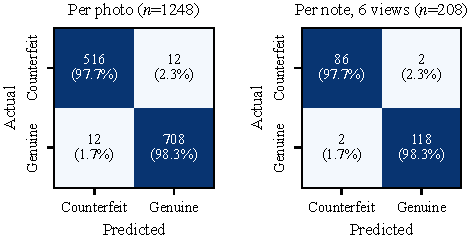
\includegraphics[width=\columnwidth]{fig_confusion}
\caption{Confusion matrices on the test split, per photograph (left) and per note after
fusing six photographs (right). Percentages are row-normalised.}
\label{fig:confusion}
\end{figure}

\begin{figure}[!t]
\centering
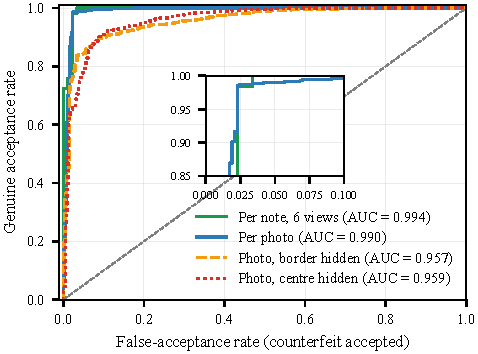
\includegraphics[width=\columnwidth]{fig_roc}
\caption{ROC curves on the test split for per-note fusion, single photographs, and the
two occlusion diagnostics of Section~\ref{sec:shortcut}. The inset magnifies the
low-false-acceptance region.}
\label{fig:roc}
\end{figure}

The per-note confusion matrix is exactly the per-photograph matrix divided by six: every
error occurs on all six photographs of the same note. The same holds for each view
position separately (all six reach 98.08\%). The errors are therefore not caused by an
unlucky photograph or viewing angle, but by four specific notes, which
Section~\ref{sec:audit} examines.

\subsection{Comparison With Baselines}
\label{sec:baselines}
To judge how much of the performance is due to fine-tuning, we evaluated two classifiers
on \emph{frozen} ImageNet EfficientNet-B0 embeddings with the same split and the same
evaluation crop: a 1-nearest-neighbour (1-NN) classifier with cosine similarity, and a
class-balanced logistic-regression linear probe. Note-level scores average the
per-photograph outputs, as in Eq.~\eqref{eq:fusion}. Table~\ref{tab:baselines} shows that
fine-tuning improves per-photograph accuracy by 1.4--1.6 points and AUC by 0.009--0.023.
At note level, however, the linear probe matches the accuracy of the fine-tuned model,
and even the 1-NN classifier errs on only six notes. For reference, the JaalTaka
authors reported 97.4--98.9\% for five fine-tuned CNNs~\cite{piyas2025jaaltaka}; their
split protocol differs from ours, so those figures are not directly comparable.

\begin{table}[!t]
\caption{Comparison With Frozen-Feature Baselines on the Test Split}
\label{tab:baselines}
\centering
\footnotesize
\setlength{\tabcolsep}{4pt}
\begin{adjustbox}{max width=\columnwidth}
\begin{tabular}{@{}lcccc@{}}
\toprule
& \multicolumn{2}{c}{Per photograph} & \multicolumn{2}{c}{Per note} \\
\cmidrule(lr){2-3}\cmidrule(l){4-5}
Method & Acc.\ (\%) & AUC & Acc.\ (\%) & AUC \\
\midrule
1-NN, frozen ImageNet features & 96.71 & 0.967 & 97.12 & 0.979 \\
Linear probe, frozen features  & 96.47 & 0.981 & 98.08 & 0.983 \\
Fine-tuned EfficientNet-B0 (ours) & \textbf{98.08} & \textbf{0.990} & \textbf{98.08} & \textbf{0.994} \\
\bottomrule
\end{tabular}
\end{adjustbox}
\end{table}

\subsection{Multi-View Fusion and the Strictness Threshold}
To measure the value of additional photographs, we evaluated Eq.~\eqref{eq:fusion} on
every subset of $k$ views of each test note ($\binom{6}{k}$ subsets per $k$).
Table~\ref{tab:views} shows that accuracy is the same for every subset, again because
all errors are note-level, whereas the mean AUC increases monotonically from 0.990 with
one photograph to 0.994 with six: fusion makes the ranking of notes more reliable and
pushes the scores of both classes further from the decision boundary.

\begin{table}[!t]
\caption{Effect of the Number of Fused Photographs (Test Notes)}
\label{tab:views}
\centering
\footnotesize
\setlength{\tabcolsep}{4pt}
\begin{adjustbox}{max width=\columnwidth}
\begin{tabular}{@{}lcccccc@{}}
\toprule
Photographs $k$ & 1 & 2 & 3 & 4 & 5 & 6 \\
\midrule
Subsets per note & 6 & 15 & 20 & 15 & 6 & 1 \\
Accuracy (\%) & 98.08 & 98.08 & 98.08 & 98.08 & 98.08 & 98.08 \\
Mean AUC & 0.9900 & 0.9912 & 0.9917 & 0.9925 & 0.9930 & 0.9939 \\
\bottomrule
\end{tabular}
\end{adjustbox}
\end{table}

Fig.~\ref{fig:scores}(a) shows that the fused scores are strongly bimodal: all
correctly classified genuine notes have $\bar{p}>0.86$ and all correctly classified
counterfeits $\bar{p}<0.10$. Consequently, the three-way rule of Eq.~\eqref{eq:decision}
leaves the outcome unchanged for $\tau\le0.85$; at $\tau=0.90$, one genuine note (0.8\%)
becomes ``uncertain'' (Fig.~\ref{fig:scores}(b)). The two accepted counterfeits have
$\bar{p}\approx0.95$ and would only be caught with $\tau>0.954$, at which point most
genuine notes would also be sent to manual inspection. The threshold therefore cannot
fix these two errors, which is consistent with the finding of Section~\ref{sec:audit}
that they are not ordinary misclassifications.

\begin{figure*}[!t]
\centering
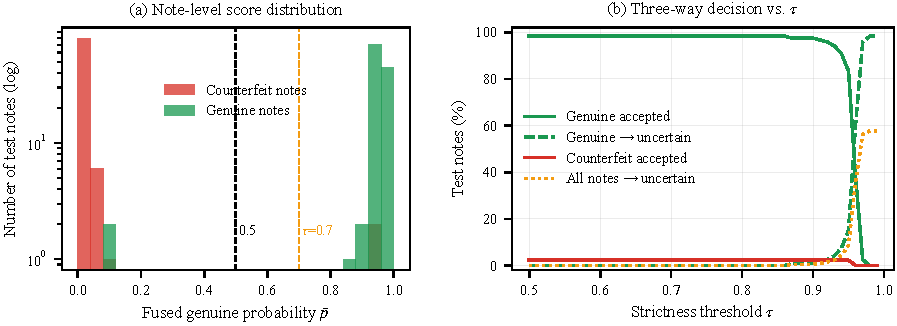
\includegraphics[width=\textwidth]{fig_scores}
\caption{(a) Distribution of the fused genuine probability $\bar{p}$ of the 208 test
notes (log scale); dashed lines mark the counterfeit limit 0.5 and the default
strictness $\tau=0.7$. (b) Share of test notes accepted as genuine, sent to
``uncertain'', or wrongly accepted, as a function of the strictness threshold $\tau$.}
\label{fig:scores}
\end{figure*}

\subsection{Out-of-Distribution Gate}
Fig.~\ref{fig:ood} shows the distribution of the OOD ratio $r(\mathbf{e})$. By
construction, about 0.5--1\% of in-distribution photographs exceed the limit: on the
test split, 4 of 1{,}248 photographs (0.32\%) are rejected, against 0.72\% on the
validation split used for calibration. The median ratio of test photographs is 0.26,
far below the limit. Because a note is analysed whenever at least one of its
photographs passes, no test note was declared ``not supported''. In a preliminary check,
the gate rejected 100 of 105 photographs of other Bangladeshi denominations (Tk~2--200)
taken from a separate collection, as well as blank, noise, and unrelated images. A
systematic OOD benchmark with independently collected images remains future work.

\begin{figure}[!t]
\centering
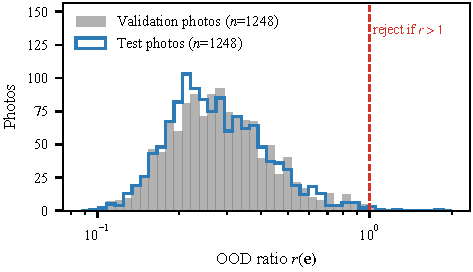
\includegraphics[width=\columnwidth]{fig_ood}
\caption{OOD ratio $r(\mathbf{e})$ of validation photographs (used for calibration) and
test photographs. Photographs to the right of the dashed line are excluded from the
note-level decision.}
\label{fig:ood}
\end{figure}

\subsection{Visual Explanations}
Fig.~\ref{fig:gradcam} shows Grad-CAM heatmaps for the genuine test note with the
highest fused score, the counterfeit note with the lowest, and one of the two accepted
counterfeits. For correct decisions, the heatmaps concentrate on the printed portrait
and on the denomination text and ornament panels, regions that carry the finest printed
detail of the note. On the counterfeit in
row~(b), the left border with the vertical security band also contributes. The heatmaps
of the wrongly accepted note in row~(c) look like those of a genuine note, which is
expected if, as shown next, an identical copy of this note appears in the training set
labelled as genuine.

\begin{figure*}[!t]
\centering
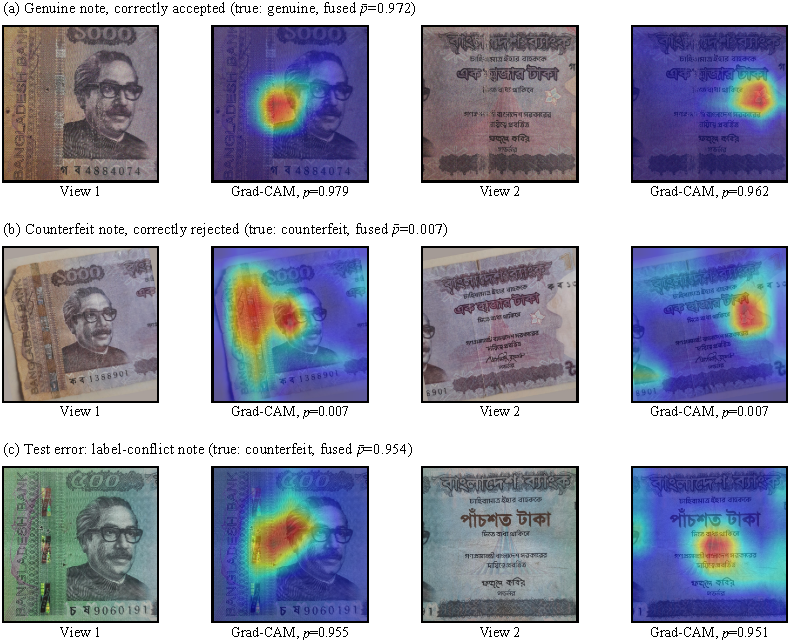
\includegraphics[width=\textwidth]{fig_gradcam}
\caption{Grad-CAM explanations on held-out test notes (views~1 and~2; red indicates
high relevance). (a)~Genuine note correctly accepted. (b)~Counterfeit note correctly
rejected. (c)~Counterfeit note wrongly accepted; its photographs also occur in the
training set under the genuine label (Section~\ref{sec:audit}).}
\label{fig:gradcam}
\end{figure*}

\subsection{Shortcut Diagnostic}
\label{sec:shortcut}
To test whether the model relies on the note or on its surroundings, we blacked out
either the central region of each test input (keeping a 20\% border) or the border
(keeping the centre), as illustrated in Fig.~\ref{fig:shortcut}, and evaluated the
unchanged model. Hiding the border reduces accuracy to 88.94\% (AUC 0.957). Hiding the
centre reduces accuracy to 75.48\%, because most genuine photographs are then rejected
(genuine acceptance 58.47\%), but the AUC remains 0.959 and 98.67\% of counterfeits are
still recognised. Information sufficient to rank most photographs correctly is therefore
present in the 20\% border alone. Part of the border is the note itself (margins,
security band, serial number), but in many photographs it also contains the table or
hand on which the note lies, and the genuine and counterfeit notes came from different
sources (banks and RAB) and were likely photographed in different sessions. We cannot rule out that capture conditions such as background,
lighting, or the phone used contribute to the decision, a classic shortcut
risk~\cite{geirhos2020shortcut}.

\begin{figure*}[!t]
\centering
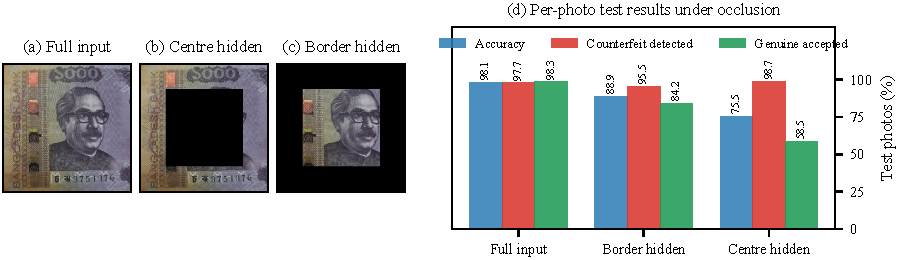
\includegraphics[width=\textwidth]{fig_shortcut}
\caption{Occlusion diagnostic. (a)--(c) Evaluation input, with the centre or the 20\%
border hidden. (d) Per-photograph test accuracy, counterfeit detection rate, and genuine
acceptance rate of the unchanged model under each condition.}
\label{fig:shortcut}
\end{figure*}

\subsection{Benchmark Audit: Duplicates and Label Conflicts}
\label{sec:audit}
The near-perfect agreement between all photographs of a note, the strength of the
non-adaptive baselines, and the statement that the dataset was enlarged by augmentation
led us to search for duplicated notes. For every pair of notes, we computed the
normalised cross-correlation (NCC) between $48\times48$ grey-scale thumbnails of
corresponding views, which is invariant to brightness and contrast changes, averaged it
over the six views, and took the maximum over horizontal and vertical flips. The
distribution of the best match is clearly bimodal (Fig.~\ref{fig:leakage}(a)): for the
validation and test notes, matches below the gap reach at most 0.963, whereas matches
above it are at least 0.997. We therefore grouped notes whose six views match with NCC $>0.98$ (connected components).
Table~\ref{tab:audit} summarises the findings.

\begin{table}[!t]
\caption{Duplicate Audit of JaalTaka (Pixel NCC $>0.98$ Over Six Views)}
\label{tab:audit}
\centering
\footnotesize
\setlength{\tabcolsep}{4pt}
\begin{adjustbox}{max width=\columnwidth}
\begin{tabular}{@{}lr@{}}
\toprule
Quantity & Value \\
\midrule
Notes / distinct photograph sets (groups) & 1{,}390 / 846 \\
Groups of size 1 / 2 / 3 & 449 / 250 / 147 \\
Notes sharing their photographs with another note & 941 (67.7\%) \\
Groups with only counterfeit / only genuine labels & 289 / 545 \\
Groups containing \emph{both} labels & 12 (31 notes) \\
\midrule
Test notes with a copy in training or validation & 116 of 208 (55.8\%) \\
\quad counterfeit / genuine & 60 of 88 / 56 of 120 \\
Test notes in label-conflict groups & 6 \\
Test errors explained by label conflicts & 4 of 4 \\
\bottomrule
\end{tabular}
\end{adjustbox}
\end{table}

\begin{figure*}[!t]
\centering
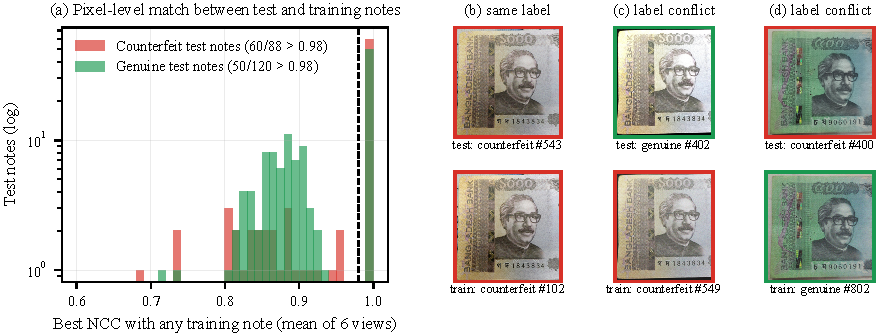
\includegraphics[width=\textwidth]{fig_leakage}
\caption{Duplicate audit. (a) Best pixel-level match (mean NCC over the six views)
between each test note and any training note; the dashed line marks the duplicate
threshold 0.98. (b)--(d) First view of a test note (top) and its matching training note
(bottom); frame colour gives the dataset label (green: genuine, red: counterfeit).
(b) An augmented copy with the same label. (c), (d) Identical photographs stored under
opposite labels.}
\label{fig:leakage}
\end{figure*}

Three findings stand out. First, the 1{,}390 notes contain only 846 distinct photograph
sets, so the augmented copies mentioned in the dataset description were stored as
independent notes. A note-level split thus places copies of 55.8\% of the test notes in
the training or validation data. Second, 12 groups contain both genuine- and
counterfeit-labelled copies of the \emph{same} photographs (e.g., genuine notes
400--406 duplicate counterfeit notes 106--112 and 547--553, and counterfeit notes 400 and
403--406 duplicate genuine notes 802 and 1--4). At least one label in each of these
groups must be wrong. The genuine-labelled notes 402 and 403, for instance, carry the
serial number 1843834, which also appears on several counterfeit-labelled notes in the
dataset. Third,
\emph{all four} test errors of our system are notes from these label-conflict groups,
and in each case the model predicts the label of the copy it saw during training.

We therefore re-scored the system and the baselines on two subsets of the original test
split (Table~\ref{tab:clean}). On the 92 \emph{clean} test notes, whose duplicate group
has no member in training or validation, all three methods are error-free. After
removing only the six label-conflict notes, all three are also error-free on the
remaining 202 notes. The reported 98.08\% note-level accuracy is thus not limited by
the model. It is the label noise of the benchmark, and on correctly labelled notes the
task is saturated even for a nearest-neighbour classifier on generic features.

\begin{table}[!t]
\caption{Note-Level Accuracy (\%) on Audited Test Subsets}
\label{tab:clean}
\centering
\footnotesize
\setlength{\tabcolsep}{4pt}
\begin{adjustbox}{max width=\columnwidth}
\begin{tabular}{@{}lccc@{}}
\toprule
Test subset & All & Without label & Clean \\
& & conflicts & (no copy) \\
\midrule
Notes (genuine / counterf.) & 208 (120/88) & 202 (117/85) & 92 (64/28) \\
\midrule
1-NN, frozen features & 97.12 & 100.0 & 100.0 \\
Linear probe, frozen & 98.08 & 100.0 & 100.0 \\
Ours (fine-tuned) & 98.08 & 100.0 & 100.0 \\
\quad 95\% Wilson CI & 95.16--99.25 & 98.13--100 & 95.99--100 \\
\bottomrule
\end{tabular}
\end{adjustbox}
\end{table}

%% ======================================================================
\section{Discussion}
\label{sec:discussion}

\subsection{What the Results Do and Do Not Show}
Within JaalTaka, the proposed system separates genuine and counterfeit notes perfectly
once label conflicts are removed, with a lower 95\% confidence bound of 96.0\% on the
92 notes that have no copy in training. Its scores are well separated, its errors are
fully explained, and it runs in real time on a CPU. These results do not, however, show
that the system will detect \emph{new} counterfeits. The 588 counterfeit notes collapse
into 289 counterfeit-only photograph sets, the counterfeits we inspected visually share
a small number of serial numbers, and they were collected separately from the genuine
notes. A model, or even a 1-NN classifier, can therefore succeed by recognising
the visual signature of known counterfeit batches or capture sessions, as the occlusion
diagnostic suggests, rather than generic evidence of forgery. Saturation also means
that the benchmark can no longer rank methods: the differences between published CNNs
on JaalTaka are smaller than the effect of its label noise.

\subsection{Recommendations for the Benchmark}
For future work on JaalTaka and similar datasets, we recommend (i)~removing or
relabelling the 12 label-conflict groups; (ii)~splitting by duplicate group, not by
note identifier, for which we release our group list; (iii)~holding out entire
counterfeit families (e.g., by serial number or seizure batch) and capture devices, to
measure generalisation to unseen forgeries and phones; and (iv)~reporting results with
confidence intervals and simple frozen-feature baselines, which immediately reveal a
saturated benchmark.

\subsection{Limitations}
The system covers only Tk~500 and Tk~1000, the denominations for which counterfeit
photographs are publicly available; other notes are answered with ``not supported''. A
visible-light photograph cannot capture ultraviolet features, magnetic ink, or the
tactile relief of intaglio print, so the output should be treated as decision support
and suspicious notes should be confirmed at a bank. Close-up phone photographs are the
only image type in the training data, and flatbed scans or distant photographs of the
whole note are mostly rejected by the OOD gate. The OOD evaluation on other
denominations is preliminary, and the class probabilities have not been calibrated on
an independent dataset~\cite{guo2017calibration}. Finally, we did not retrain the model
on a group-aware split; doing so, together with a counterfeit-family hold-out, is the
most important next step.

%% ======================================================================
\section{Conclusion}
\label{sec:conclusion}

We presented a reliability-oriented smartphone system for detecting counterfeit
Bangladeshi Tk~500 and Tk~1000 notes. It combines a fine-tuned EfficientNet-B0,
fusion of up to six photographs, a three-way decision with adjustable strictness, an
embedding-space OOD gate, and Grad-CAM explanations, and it runs in real time on a
CPU. On a note-disjoint JaalTaka test split, it achieves 98.08\% note-level accuracy
and an AUC of 0.994. A pixel-level audit showed that this figure mainly reflects the
benchmark: most test notes have copies in the training data, 12 duplicate groups carry
contradictory labels, and these conflicts explain every test error, while on
duplicate-free notes even simple baselines are error-free. Progress in counterfeit
detection now depends less on new architectures than on evaluation data that separates
counterfeit families, capture sessions, and devices, and on reliability mechanisms such
as those proposed here.

%% ======================================================================
\section*{Acknowledgment}
The authors thank the Department of Software Engineering, Daffodil International
University, for laboratory facilities and administrative support, and the creators of
the JaalTaka dataset for making their data publicly available. This research received
no external funding.

\section*{Author Contributions}
D.~Biswas: conceptualisation, software, experiments, formal analysis, and writing of the
original draft. I.~Mahmud: supervision, methodology review, and review and editing of
the manuscript.

\section*{Conflict of Interest}
The authors declare that they have no conflict of interest.

\section*{Generative AI Disclosure}
%% TODO (authors): adapt this statement to the journal's policy and to how AI tools
%% were actually used.
The authors used an AI assistant to help write analysis and plotting scripts and to
edit the manuscript text. The authors checked all code, results, and references and take
full responsibility for the content of this paper.

\section*{Data and Code Availability}
The JaalTaka dataset is publicly available from Mendeley Data under the CC~BY~4.0
licence~\cite{jaaltaka_data}. The trained model, the training and evaluation code, the
scripts that reproduce every table and figure, and the list of duplicate groups found in
the audit are available from the corresponding author and will be released in a public
repository upon publication.

%% ----------------------------------------------------------------------
\bibliographystyle{IEEEtran}
\bibliography{references}

%% ----------------------------------------------------------------------
%% Biographies. TODO (authors): complete them, or delete this block if the
%% journal does not ask for biographies. To add a photo, use
%% \begin{IEEEbiography}[{\includegraphics[width=1in,height=1.25in,clip,keepaspectratio]{photo.jpg}}]{Name}
\begin{IEEEbiographynophoto}{Debobrato Biswas}
is with the Department of Software Engineering, Daffodil International University,
Dhaka, Bangladesh. % TODO: degrees, research interests, IEEE membership.
\end{IEEEbiographynophoto}

\begin{IEEEbiographynophoto}{Imran Mahmud}
is with the Department of Software Engineering, Daffodil International University,
Dhaka, Bangladesh. % TODO: degrees, positions, research interests.
\end{IEEEbiographynophoto}

\end{document}
